% Section content template for individual Educative lessons
% This file contains the actual content for a specific section
% Generated from Educative API section content

% Section: AI Evaluation of Building Blocks in E-Commerce Platform
% Section ID: 5469233437868032
% Section Slug: ai-evaluation-of-building-blocks-in-e-commerce-platform
% Generated: 2025-12-07T22:22:08.564561

In this lesson, we will assess our understanding of building blocks using an AI interactive widget. Let's begin!

\subsection{An e-commerce platform}\label{UGTumc77vSDddmlkH8KG9}
\\
Consider an abstract and simplified system design for an e-commerce platform outlined below. The design comprises various components that collaborate to execute diverse tasks. The customer engages with multiple services such as search, shopping cart, and order-taking services. While details for each component and service in the design have been provided, some missing components are not described. Your objective is to identify these missing components and concisely describe their functions using the AI interactive widget given at the end of the lesson.

\begin{figure}[htbp]
 \centering
 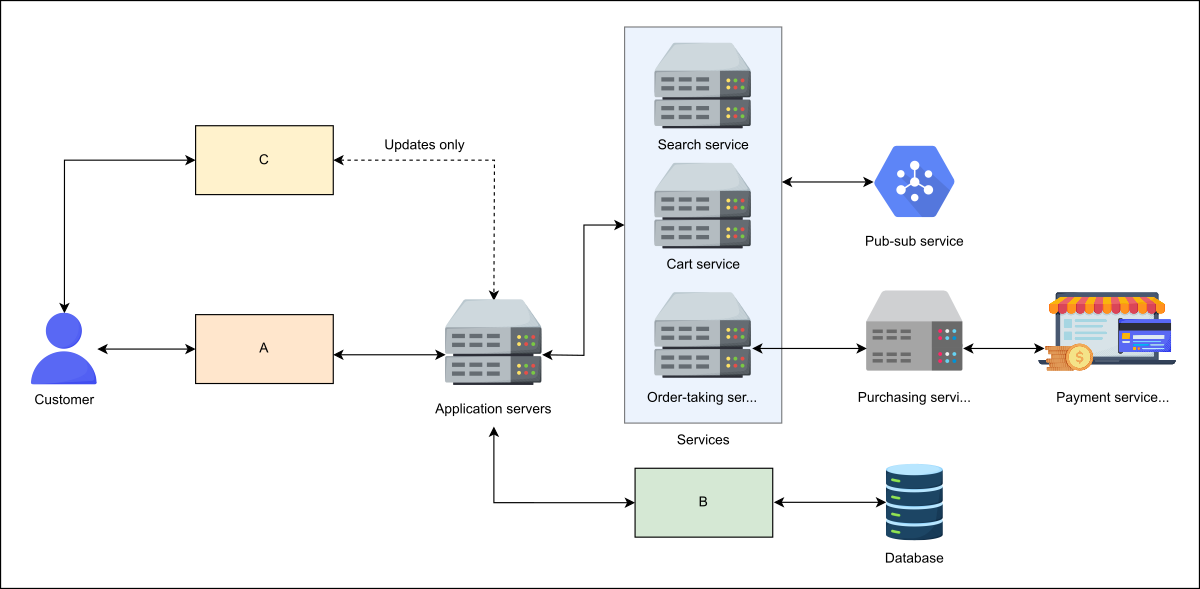
\includegraphics[width=0.5\textwidth]{Images/chapter_25/section_5469233437868032/4994640858447872.png}
 \caption{A high-level design of the e-commerce platform}
\end{figure}

Different components in the design are described below:

\begin{enumerate}
\item
\protect\phantomsection\label{FEWdnetaRrmtZxjmXPMdf}
\textbf{Application servers:} They provide middleware services by facilitating communication between different components of an application. They also forward user queries to the respective services.
\item
\protect\phantomsection\label{h0HVi01RyOU7FxXxZXMXF}
\textbf{Search service:}~This component handles search queries requested by users.
\item
\protect\phantomsection\label{cWFO9QcYRmASYSWXbhB09}
\textbf{Cart service:}~This service handles the shopping cart where the customers select different products to purchase.
\item
\protect\phantomsection\label{NUjCB5g8IrksGIK_lqgQu}
\textbf{Order-taking service:~} This service initiates customer orders, triggering the purchasing service upon the user's request.
\item
\protect\phantomsection\label{Q53yg4lkf7k8NWdKbRtx8}
\textbf{Payment service provider (PSP):}~The PSP handles payment transactions securely, interacting with external payment gateways.
\item
\protect\phantomsection\label{KuXozvAQflYJzS2xI2FuY}
\textbf{Database:}~It stores the user and product information, such as images, prices, descriptions, and other metadata permanently.
\end{enumerate}
\\
Your task is to determine the missing components A, B, and C in the above design. You need to provide your answer in the correct order (A, B, and then C) along with a concise description.

\textbf{Question:}

Find the missing building blocks in the e-commerce system design.

\textbf{Reference Answer:}

Component A = load balancers that distribute incoming traffic across multiple servers. Component B = the caching layer, which optimizes performance by storing frequently accessed data. It can also be referred to as a distributed cache. Component
C = a Content Delivery Network (CDN) used for optimizing the delivery of static assets like images and stylesheets. It also enhances website performance by serving static content from strategically distributed servers. CDNs get updated content from the origin servers, which, in this case, are application servers.



% End of section content